\section{Clase 31}
Considerando $B=0$, ¿puede existir una magnetización espontánea?. Considerendos el promedio de $\s_i$,
\begin{equation}
  \ev{\s_i}\equiv \frac{\sum_{i=1}^N\s_i}{(N-1)}
\end{equation}
considerando $N$ spines en total. El $N-1$ se introduce para segurar que $N>1$.

\subsection{Aproximación de campo medio}
Estudiamos un spin $i$. Todos los spines, excepto $i$ tienen su valor promedio $\ev{\s}$. Luego, el Hamiltoniano para el spin $i$ se puede escribir como
\begin{equation}
  H_i=-qJ\ev{\s }\s_i-\m B\s_i
\end{equation}
donde $q$ es el número de vecinos cercanos por spin.

\begin{ej}
Consideremos el siguiente sistema
	\begin{figure}[h!]
	\centering
	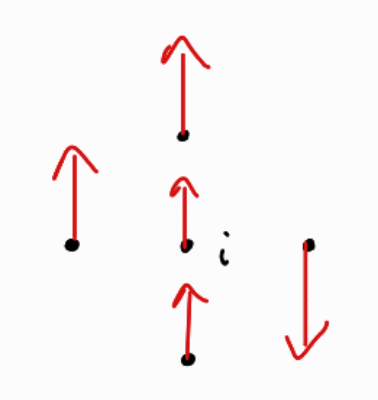
\includegraphics[scale=0.5]{fig/spin}
\end{figure}

vemos que$\ev{\s}=1/2$. Luego,
\begin{equation}
  H_i=-2J-\m B
\end{equation}
La probabilidad de que el spin $i$ tenga la orientación $\s_i$ vendrá dada por el factor de Boltzman usual
\begin{equation}
  P(\s_i)=\frac{e^{-\b H_i(\s_i )}}{\zc }
\end{equation}
El valor promedio será
\begin{equation}
  \ev{\s_i}=\sum_{\s_i=\pm 1}\s_iP(\s_i)
\end{equation}
donde 
\begin{equation}
  \zc=\sum_{\s_i=\pm 1} e^{-\b H_i(\s_i)}
\end{equation}
Exlplícitamente
\begin{align}
  H_i(\s_i=1)&=-qJ\ev{\s}-\m B\\
  H_i(\s_i=-1)&=qJ\ev{\s}+\m B
\end{align}
entonces 
\begin{equation}
  \zc=e^{\b(qJ\ev{\s}+\m B)}+e^{-\b(qJ\ev{\s}+\m B)}
\end{equation}
Ahora
\begin{align}
  P(\s_i=1)&=\frac{e^{\b(qJ\ev{\s}+\m B)}}{\zc }\\
   P(\s_i=-1)&=\frac{e^{-\b(qJ\ev{\s}+\m B)}}{\zc }
\end{align}
Finalente,
\begin{equation}
  \ev{\s_i}=\frac{e^{\b(qJ\ev{\s}+\m B)}-e^{-\b(qJ\ev{\s}+\m B)}}{e^{\b(qJ\ev{\s}+\m B)}+e^{-\b(qJ\ev{\s}+\m B)}}=\tanh (\b(qJ\ev{\s}+\m B))
\end{equation}
Ahora, como ningun spin es epecial respecto a los demas, por consistencia lógica, en la configuración de equilibrio se tiene
\begin{equation}
  \ev{\s_i}=\ev{\s}
\end{equation}
Luego, se obtiene una ecuación algebraica para $\s$,
\begin{equation}
 \boxed{ \ev{\s}=\tanh (\b(qJ\ev{\s}+\m B))}
\end{equation}
En la aproximación de campo medio, puedo encontrar $\ev{\s}$ en cualquier dimensión y con cualquier topología de conectividad, analizando un único spin.
\end{ej}

\textbf{Caso B=0}
Se tiene
\begin{figure}[h!]
	\centering
	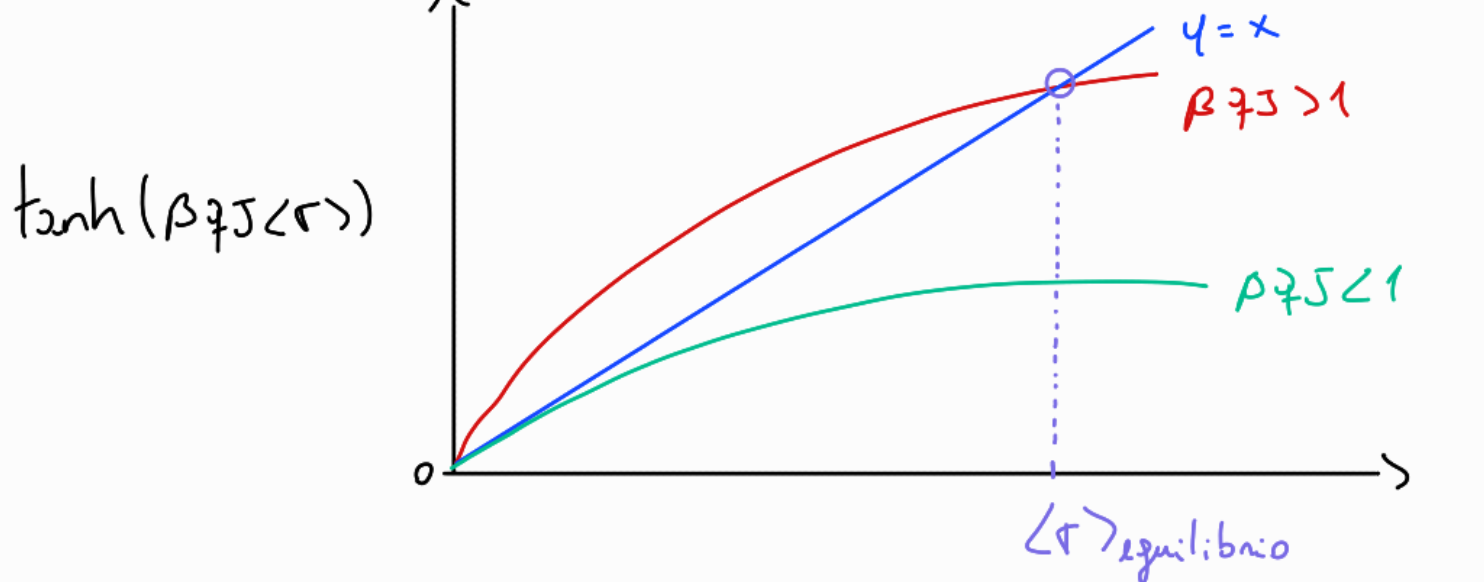
\includegraphics[scale=0.4]{fig/31-gra}
\end{figure}

Para $\b qJ>1$, existen dos soluciones
\begin{equation}
  \ev{\s}=\ev{\s}_{\rm equilibrio}\neq 0,\qquad \ev{\s}=0
\end{equation}

Para $\b qJ<1$, la única solución es $\ev{\s}=0$.

Notemos que $qJ/(\k T_c)=1$ define la temperatura crítica para la cual comienza a existir magnetización espontánea, es decir,
\begin{equation}
  \boxed{T_c=\frac{qJ}{\k }}
\end{equation}
donde para $T<T_c$ hay magnetiación espontánea y para $T>T_c$ o hay magnetización espontánea.

Gráficamente esto se ve como
\begin{figure}[h!]
	\centering
	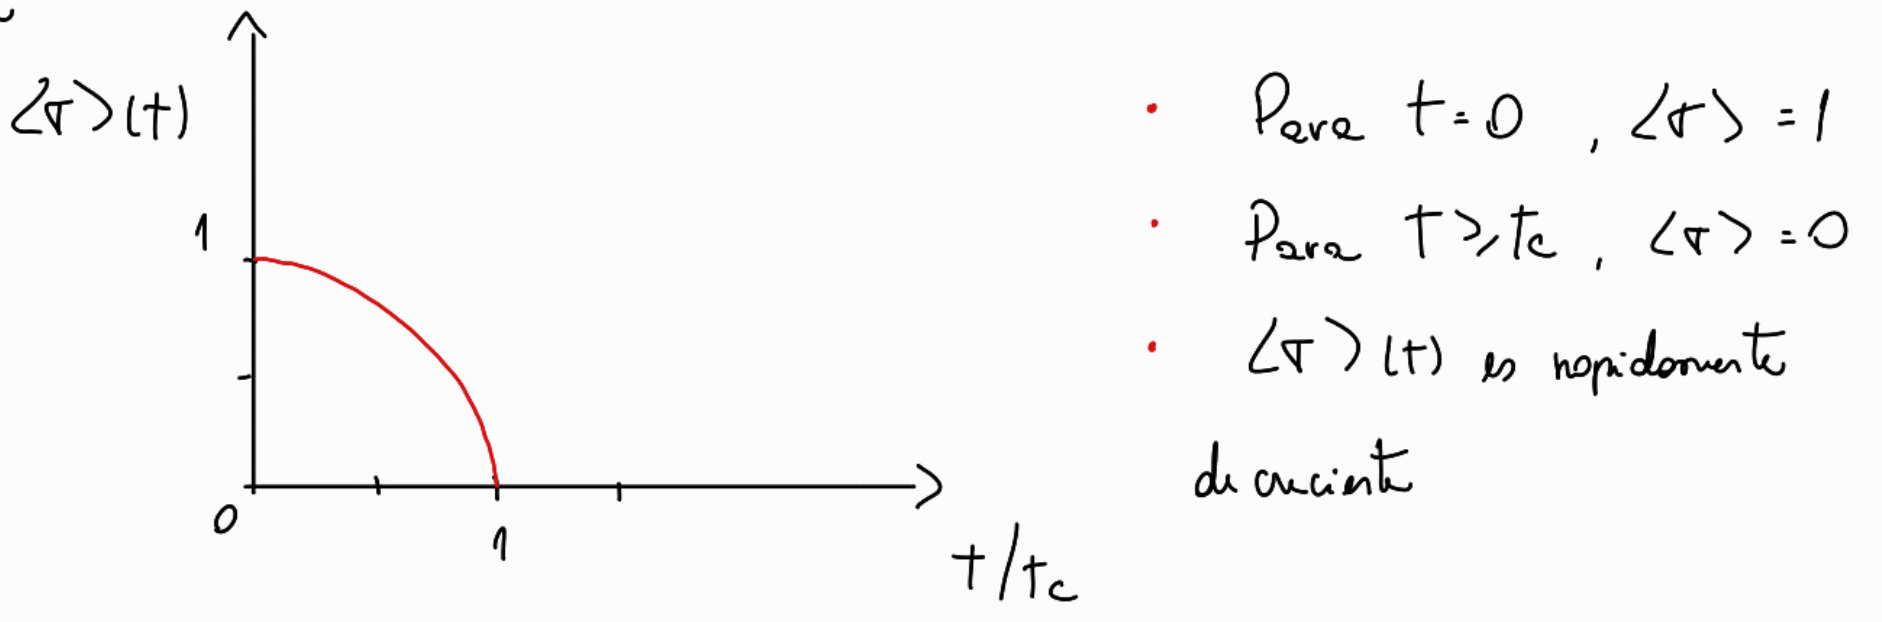
\includegraphics[scale=0.4]{fig/31-es}
\end{figure}










































